\documentclass[twoside]{article}
\usepackage{amsmath,amssymb}
\usepackage[utf8]{inputenc}
\usepackage[spanish]{babel}
\usepackage{caption}
\usepackage[]{graphicx}
\usepackage{enumerate}
\usepackage{amsthm}
\usepackage{tikz-cd}
\usetikzlibrary{babel}
\usepackage{pgf,tikz}
\usepackage{mathrsfs}
\usepackage{bm}  
\usetikzlibrary{arrows}
\usetikzlibrary{cd}
\usepackage[spanish]{babel}
\usepackage{fancyhdr}
\usepackage{titlesec}
\usepackage{floatrow}
\usepackage{makeidx}
\usepackage[tocflat]{tocstyle}
\usetocstyle{standard}
\usepackage{subfiles}
\usepackage{color}  
\usepackage{hyperref}
\hypersetup{colorlinks=true,citecolor=red, linkcolor=blue}
\usepackage{eurosym}
%\usepackage{ntheorem}


\renewcommand{\baselinestretch}{1,4}
\setlength{\oddsidemargin}{0.25in}
\setlength{\evensidemargin}{0.25in}
\setlength{\textwidth}{6in}
\setlength{\topmargin}{0.1in}
\setlength{\headheight}{0.1in}
\setlength{\headsep}{0.1in}
\setlength{\textheight}{8in}
\setlength{\footskip}{0.75in}

\theoremstyle{definition}

\newtheorem{teorema}{Teorema}[section]
\newtheorem{defi}[teorema]{Definición}
\newtheorem{coro}[teorema]{Corolario}
\newtheorem{lemma}[teorema]{Lema}
\newtheorem{ej}[teorema]{Ejemplo}
\newtheorem{ejs}[teorema]{Ejemplos}
\newtheorem{observacion}[teorema]{Observación}
\newtheorem{observaciones}[teorema]{Observaciones}
\newtheorem{prop}[teorema]{Proposición}
\newtheorem{propi}[teorema]{Propiedades}
\newtheorem{nota}[teorema]{Nota}
\newtheorem{notas}[teorema]{Notas}
\newtheorem*{dem}{Demostración}
\newtheorem{ejer}[teorema]{Ejercicio}
\newtheorem{problem}[teorema]{Problema}
\newtheorem{concl}[teorema]{Conclusión}

\providecommand{\abs}[1]{\lvert#1\rvert}
\providecommand{\sen}[1]{sen #1}
\providecommand{\norm}[1]{\lVert#1\rVert}
\providecommand{\ninf}[1]{\norm{#1}_\infty}
\providecommand{\numn}[1]{\norm{#1}_1}
\providecommand{\gabs}[1]{\left|{#1}\right|}
\newcommand{\bor}[1]{\mathcal{B}(#1)}
\newcommand{\R}{\mathbb{R}}
\newcommand{\Z}{\mathbb{Z}}
\newcommand{\N}{\mathbb{N}}
\newcommand{\Q}{\mathbb{Q}}
\newcommand{\C}{\mathbb{C}}
\newcommand{\Pro}{\mathbb{P}}
\newcommand{\Tau}{\mathcal{T}}
\newcommand{\verteq}{\rotatebox{90}{$\,=$}}
\newcommand{\vertequiv}{\rotatebox{110}{$\,\equiv$}}
\providecommand{\lrg}{\longrightarrow}
\providecommand{\func}[2]{\colon{#1}\longrightarrow{#2}}
\newcommand*{\QED}{\hfill\ensuremath{\blacksquare}}
\newcommand*\circled[1]{\tikz[baseline=(char.base)]{
            \node[shape=circle,draw,inner sep=1.5pt] (char) {#1};}}
\newcommand*{\longhookarrow}{\ensuremath{\lhook\joinrel\relbar\joinrel\rightarrow}}


\begin{document}
%\title{Topología de Superficies}
%\author{Antonio Rafael Quintero Toscano\\ Javier Aguilar Martín}
%\date{Curso 2016/2017}
%\maketitle

\author{Javier Aguilar Martín y Rafael González López}
\date{\today}
\title{La criptografía detrás de Bitcoin}

\maketitle

\begin{figure}[h!]
		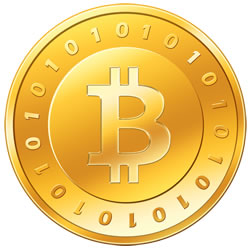
\includegraphics[scale=0.7]{bitcoin.jpg}
\end{figure}

\begin{abstract}
    En este trabajo vamos a explorar el funcionamiento interno de Bitcoin, la criptomoneda más famosa y más valorada. Para ello, empezaremos presentando informalmente qué es Bitcoin y explicando los conceptos criptográficos previos que serán necesarios para entender el resto del trabajo. A continuación entraremos en detalle en los algoritmos usados por Bitcoin para poder considerarse funcional y seguro. Por último comentaremos algunas otras aplicaciones de las ideas que subyacen a esta moneda.
\end{abstract}


	\vfill
	Esta obra está licenciada bajo la Licencia Creative Commons Atribución 3.0 España. Para ver una copia de esta licencia, visite \url{http://creativecommons.org/licenses/by/3.0/es/} o envíe una carta a Creative Commons, PO Box 1866, Mountain View, CA 94042, USA.


\newpage
\tableofcontents

\newpage


\section{Preliminares}

\subsection{¿Qué es Bitcoin?}

Bitcoin (abreviado BTC) es una criptomoneda o criptodivisa, es decir, un medio de intercambio digital que usa las herramientas de la criptografía para garantizar la seguridad y el anonimato. Bitcoin no es la única criptomoneda existente, pero sí que fue la primera que empezó a operar en el año 2009. Algo que diferencia a esta moneda del dinero fiduciario (dinero usual) es su descentralización, ya que no existe un Banco Central de Bitcoin. Por ello no se puede manipular la cantidad total de Bitcoin existente, que está previamente fijada y es pública. Bitcoin a su vez se puede dividir en unidades menores hasta una fracción de $10^{-8}$ BTC llamada Satoshi (en honor a su creador, Satoshi Nakamoto).\\

Actualmente es reconocida como legal en varios países como Alemania o Japón, mientras que en otros como Bolivia está explíticamente prohibido. En muchos otros existe un vacío legal. Su valor a día de hoy alcanza los 1600\euro/BTC, lo cual lo convierte en un poderoso activo financiero. \\

Se puede conseguir este tipo de dinero intercambiándolo por bienes y servicios (como cualquier otro dinero) a través de un monedero o \emph{wallet}, o bien obtenerlos directamente \emph{minando} (por analogía al oro). Los procesos de intercambio y obtención de Bitcoin serán explicados más detalladamente en secciones posteriores. Antes de eso, aclararemos algunos conceptos que serán utilizados más adelante. 

\subsection{Funciones hash.}
\begin{defi}
\begin{defi}
Para un $n$ fijo, llamamos \textbf{función hash} a una función $h : \mathcal{M} \to (\mathbb{F}_2)^n$ tal que:
\begin{itemize}
	\item $h$ es resistente a preimagen: Dado $y=h(x)$ es computacionalmente infactible calcular $x$ (es \emph{one way}).
	\item $h$ es resistente a colisiones: Es computacionalmente infactible calcular $x$ y $x'$ con $h(x) = h(x')$
	\item $h$ es resistente a segunda preimagen: Dado $y=h(x)$, es computacionalmente infactible calcular $x'$ con $h(x')=y$.  
\end{itemize}
\end{defi}
Al texto recibido se le suele llamar \textbf{input} o \textbf{mensaje}, mientras que el texto devuelto se puede llamar \textbf{output} o \textbf{digest}. Normalmente el digest se expresa en hexadecimal con 40 caracteres. 
\end{defi}
Algunos ejemplos de funciones hash son SHA1, CRC32 o SHA256. Uno podría preguntarse con qué frecuencia se producen colisiones, es decir, que dos entradas de texto tengan un mismo hash. En el caso del SHA1, si tenemos $1,71\times 10^{17}$, ¿cuál es la probabilidad de que tengamos una colisión? Tan solo $1$ entre $100$ billones, es decir, la misma que tu casa sea destruida por un impacto de meteorito.

Estas funciones tienen la propiedad de que un pequeño cambio en el mensaje recibido genera una salida totalmente distinta, lo que las vuelve impredecibles, como podemos observar en el siguiente ejemplo.
	
\begin{ej}\
En este ejemplo vemos el funcionamiento de la función SHA1. 
\begin{figure}[h!]
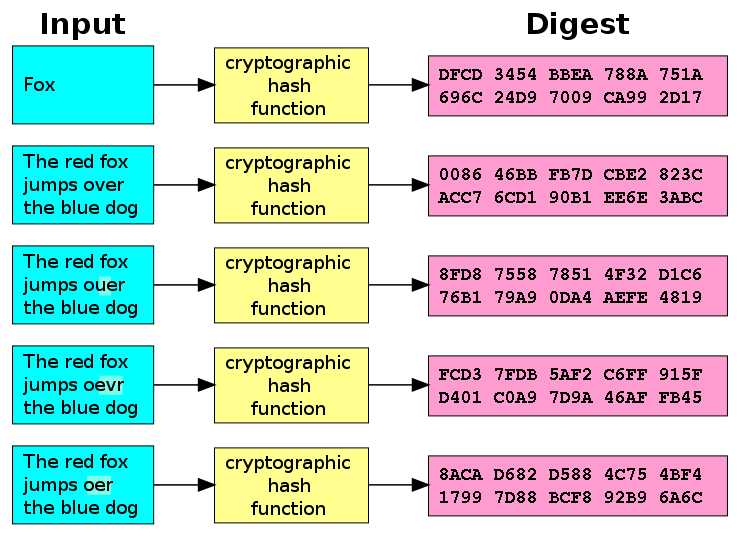
\includegraphics[scale=0.4]{hashexample}
\end{figure}
\end{ej}

No todas las funciones hash son seguras\footnote{SHA1 es un ejemplo de esto \url{https://shattered.io/}}, pero la que usa Bitcoin, SHA256, es una de las más seguras que existen.

\newpage

\subsection{Curvas elípticas.}
\begin{defi}
Una \textbf{curva elíptica} es una curva plana representada algebraicamente como una ecuación de la forma $y=x^3+ax+b$. 
\end{defi}

\begin{ej} Para $a=0$ y $b=7$, que es la que usa Bitcoin, tiene esta forma:
\begin{figure}[h!]
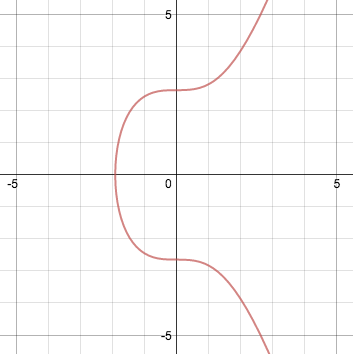
\includegraphics[scale=0.42]{ec}
\end{figure}
\end{ej}

Los puntos de una curva elíptica tiene la propiedad de que forman un grupo si definimos una suma particular que vamos a ver a continuación. 

\subsubsection{Suma en una curva elípitca.}

Para sumar dos puntos $P$ y $Q$ pertenecientes a la curva elíptica, en primer lugar tenemos que trazar la recta que pasa por dichos puntos y hallar la intersección de esta recta con la curva elíptica, al que llamaremos $R'$. Después debemos hacer una reflexión del punto de intersección con respecto al eje de abscisas (obsérvese que las curvas elípticas son simétricas con respecto a este eje). El punto obtenido es $R=P+Q$. Lo vemos más claramente en la siguiente imagen: 
\begin{figure}[h!]
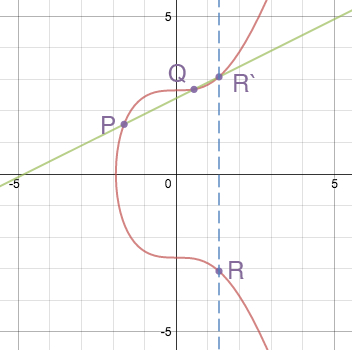
\includegraphics[scale=0.4]{sumec}
\end{figure}

En el caso de que queramos sumar un punto $P$ consigo mismo debemos hacer la operación anterior considerando la recta tangente a la curva $y$ en $P$ como se observa en la siguiente imagen:

\begin{figure}[h!]
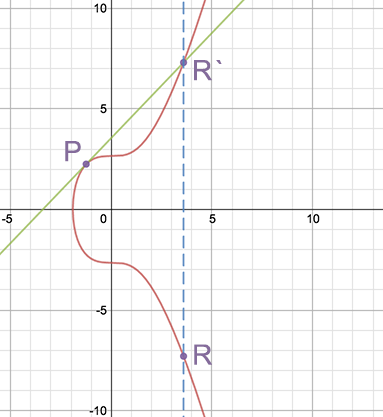
\includegraphics[scale=0.4]{pmasp}
\end{figure}

Como elemento neutro deberemos considerar al punto del infinito de la curva. Se puede observar que el inverso de un punto sería su simétrico con respecto al eje de abscisas. De forma natural se define el producto por escalar $\alpha P$ siempre que $\alpha\in\Z$ como la suma de $\alpha$ veces $P$ (o de su inverso si $\alpha<0$). Estas propiedades dotan a las curvas elípticas estructura de grupo.

\subsubsection{Curvas elípticas sobre cuerpos finitos.} 
Realmente Bitcoin no usa la curva anterior sobre $\R$ tal como la hemos dibujado, sino sobre un cuerpo finito módulo $2^{256} – 2^{32} – 2^9 – 2^8 – 2^7 – 2^6 – 2^4 - 1$, que es primo. Además se selecciona un punto base para hacer las operaciones que tiene como orden un primo lo suficientemente grande. Tanto estos parámetros como la curva son los mismos para todos los usuarios. Por visualizar qué aspecto tiene una curva elíptica sobre un cuerpo finito, observémos este ejemplo en el que se toma como primo el número $67$:
\begin{figure}[h!]
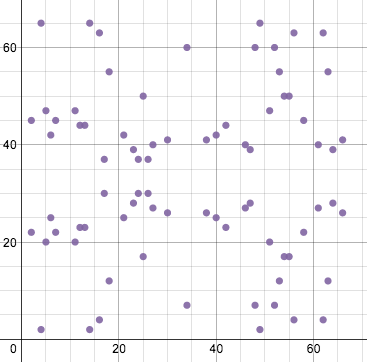
\includegraphics[scale=0.38]{field}
\end{figure}

\newpage

A pesar de lo diferente que se ve, conserva las propiedades esenciales del caso anterior. Además sigue siendo simétrica. La suma también cambia visualmente como podemos ver en esta imagen en la que sumamos $(2,22)+(6,25)$:
\begin{figure}[h!]
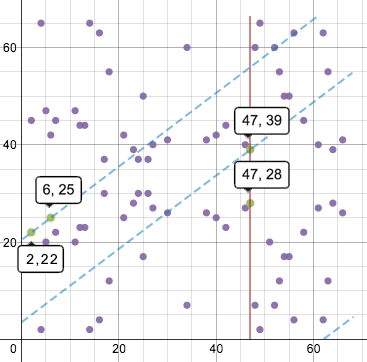
\includegraphics[scale=0.45]{sumfield}
\end{figure}

Con esto terminamos los preliminares y pasamos a explicar cómo funciona Bitcoin.
\newpage
\section{Funcionamiento interno de Bitcoin.}
\subsection{Transacciones, validación y firma.}
Comencemos precisamente el concepto de transacción, la operación fundamental en el funcionamiento de Bitcoin. 
\begin{defi} Una \textbf{transacción} es un movimiento de Bitcoin de una direccion de origen a una dirección de destino. 
\end{defi}
Cada dirección de Bitcoin representa una clave pública. Para gastar Bitcoin es necesario conocer la clave privada asociada a la clave publica que contenga un saldo en Bitcoins. Entonces, se pueden gastar esos Bitcoins, es decir, transferirlos a otra dirección, firmando digitalmente con la clave privada la transmisión de esta información y enviando la nueva transacción a toda la red, la cuál está compuesta por nodos.
\begin{defi}
Los \textbf{nodos} de Bitcoin son las entidades que forman parte del protocolo distribuido para crear un registro común de información. Cada vez que se realiza una transacción, esta se envía a todos los nodos. Por ello, tienen la tarea de validar, afianzar, transmitir y almacenar. Esto se hará con ayuda de una base de datos llamada \emph{blockchain}, que veremos más adelante.
\end{defi}
\begin{figure}[h!]
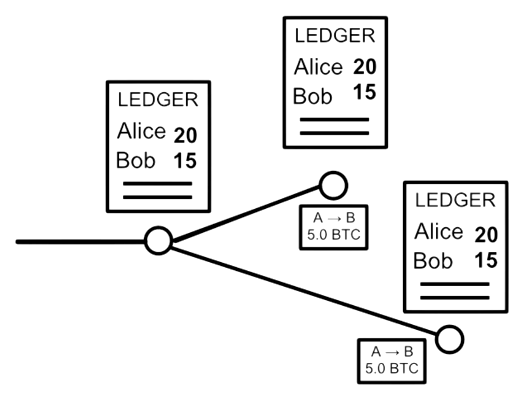
\includegraphics[scale=0.45]{transaction}
\end{figure}
Ahora vamos a ver detalladamente en qué consiste una transacción. 

Supongamos que Alice quiere enviar $5$ BTC a Bob. Para ello, Alice debe probar que tiene ese dinero y para ello el total de transacciones que haya realizado anteriormente debe sumar al menos esos $5$ Bitcoins. Las transacciones usadas como referencia se llaman \emph{inputs}. Los nodos que vayan a verificar la transacción deben comprobar los inputs para asegurar que Alice era la receptora y que la suma asciende al menos a la cantidad que desea enviar.
\begin{figure}[h!]
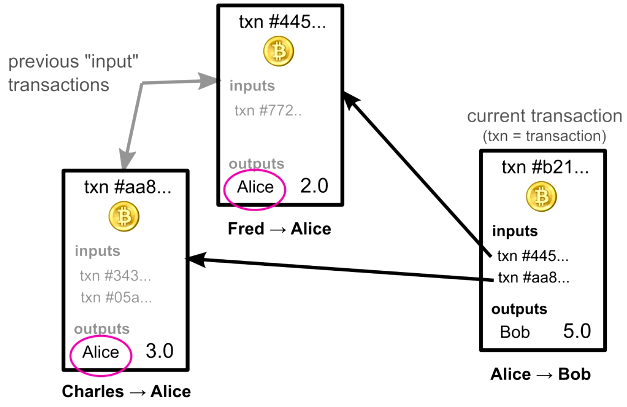
\includegraphics[scale=0.4]{inputs}
\end{figure}

Cada input debe usarse completamente, por lo que si se desea enviar una cantidad que no coincide exactamente con ninguna suma de transacciones previas se devolverá la ``vuelta'' como un segundo output además del dinero enviado a Bob. 

A través de estas referencias a transacciones pasadas, la propiedad de Bitcoins se basa en una cadena de transacciones (veremos más adelante que es la cadena de bloques). Al instalar por primera vez un monedero de Bitcoin, el software comprueba automáticamente todas las transacciones anteriores para asegurarse de tener un registro fidedigno.

Una vez que una transacción ha sido usada como referencia se considera gastada y no puede volverse a usar. De otro modo podría cometer \textbf{doble gasto} aludiendo a la misma transacción varias veces. Por lo tanto, al validar una transacción también se comprueba que las transacciones no habían sido usadas antes. Debido a que las transacciones en la red de Bitcoin se cuentan por decenas de millones, se aligera el proceso mediante un índice de transacciones no usadas. En definitiva, tener Bitcoins significa que hay una lista de transacciones que apuntan a tu dirección y que no han sido gastadas.

Ahora que hemos dejado clara la idea general de cómo se produce una transacción, volvamos a la operación que quería realizar Alice. Sean $(PK_A,SK_A)$ y $(PK_B,SK_B)$ los pares de calve pública-privada de Alice y Bob respectivamente. La función $Add(PK)$ nos devuelve la dirección generada a partir de la clave pública $PK$ aplicándole una función hash y añadiéndole delante un $1$ o un $3$ (esto se hace simplemente para indentificarlo como dirección pública de Bitcoin). Además será necesaria una firma digital, que explicaremos posteriormente, y que denotaremos $Sign_{SK}(m)$ donde $m$ representa la transacción (ya que esta firma varía en cada transacción). Sea $H$ una función hash. Supongamos que Alice ya había recibido la cantidad de $5$ BTC en una transacción $T_0$ a su dirección, $Add(PK_A)$.  Como hemos explicado antes, $T_0=\{input_0, output_0\}$. En este caso $input_0$ sería el registro anterior de transacciones y $output_0=\{Add(PK_A),5\}$. 

Para enviar el dinero a Bob, Alice necesita crear una nueva transacción $T_1$ de la siguiente forma:
\begin{align*}
&T_1=\{input_1,output_1\}\\
&input_1=\{H(T_0),Sign_{SK_A}(T_0+input),PK_A\}\\
&output_1=\{Add(PK_B),5\}
\end{align*}

Veamos por qué aparece cada uno de los términos en el $input_1$. En primer lugar, $H(T_0)$ es un hash de la transacción y actúa como puntero en la cadena de bloques como se verá en secciones posteriores. Después, se genera una nueva firma digital que solo se puede realizar con la clave privada $SK_A$ que solo posee Alice. Por último es necesario que aparezca la clave pública de Alice para poder validar la transacción y comprobar que efectivamente era dinero proveniente de su dirección. 

En el $output_1$ simplemente se indica a quién va dirigida la cantidad que se especifica, de forma que solo Bob podrá gastar esta cantidad en transacciones posteriores. Bob puede verificar que le han sido transferidos los fondos comprobando que $Add(PK_A)$ coincide con la dirección de destino de $T_0$ y también que la firma es correcta $Sign_{SK_A}(T_0+input)$ usando $PK_A$. 

Bitcoin permite realizar operaciones más complejas, como transacciones que requieren varias claves privadas, pero la base de todo es lo que hemos explicado. Nos queda pendiente mostrar cómo se calcula la firma digital.

\subsubsection{Algoritmo de firma digital en curvas elípticas. }

Para poder firmar primero se necesita tener las claves. El procedimiento por el cual se generan es ElGamal sobre una curva elíptica, que funciona de la misma forma que en cualquier otro grupo, pero con las operaciones explicadas en la primera sección.  Por ello no vamos a detallar el proceso, pero sí vamos a señalar sus pasos. 

En primer lugar se fija un \textbf{punto base} en la curva, llamémoslo $P$ de orden $N$ un primo bastante grande. Se elige como clave privada un número aleatorio $x\in\{1,\dots, N-1\}$. A partir de este, claculamos la clave pública $Y=xP$. Esto indica que el número máximo de claves públicas (y por tanto de direcciones) es justamente el orden de $P$. 

Debido a la complejidad computacional de la suma en curvas elípticas, es factible clacular la clave pública a partir de la clave privada y el punto base, pero es infactible calcular la clave privada a partir de la clave pública y el punto base. 

En Bitcoin, tanto el punto base como su orden se representan como un \emph{string} hexadecimal. Concretamente:
\begin{itemize}
\item Punto base: B04 79BE667E F9DCBBAC 55A06295 CE870B07 029BFCDB 2DCE28D9 \\59F2815B 16F81798 483ADA77  26A3C465 5DA4FBFC 0E1108A8 FD17B448 A6855419 \\ 9C47D08F FB10D4B8
\item Orden:  FFFFFFFF FFFFFFFF FFFFFFFF FFFFFFFE BAAEDCE6 AF48A03B BFD25E8C D0364141
\end{itemize}

Así pues, las claves también se representarán de este modo. Ahora que ya tenemos las claves, podemos empezar a firmar. Sea pues $P$ el punto base, $N$ su orden, $x$ la clave privada, $m$ un mensaje que vamos a firmar y $h$ una función hash que se usa para que el mensaje tenga el mísmo número de bits (256) que el orden de $P$. El algoritmo de la firma digital consiste en lo siguiente:
\begin{enumerate}
\item Calcular $e=h(m)$.
\item Sea $z$ el conjunto de $l$ dígitos más a la izquierda de $e$, donde $l$ es la longitud en bits de $N$.
\item Elegir un número entero aleatorio $k\in\{1,\dots,N-1\}$.
\item Calcular el punto $(a,b)=kP$ usando la multiplicación por escalar de la curva elíptica. 
\item Encontrar $r\equiv a\mod N$. Si $r=0$, vuelta al paso 1.
\item Encontrar $s\equiv (z+rx)k^{-1}\mod N$. Si $s=0$, vuelta al paso 1. 
\item La firma es el par $(r,s)$. 
\end{enumerate}

Es importante que $k$ sea diferente en cada firma para evitar la posibilidad de extraer la clave privada\footnote{Un error de este tipo fue usado en 2010 para extraer las claves de PS3 \url{https://nakedsecurity.sophos.com/2012/10/25/sony-ps3-hacked-for-good-master-keys-revealed/}}, ya que el resto de datos son conocidos. Dadas dos firmas $(r,s)$ y $(r,s')$ en las que se ha utilizado la misma $k$ para dos mensajes conocidos $m$ y $m'$, un atacante puede utilizar la ecuación en el paso 6 para calcular $k$, ya que $s-s'\equiv k^{-1}(z-z')\mod N$. El atacante puede hallar entonces $k=\frac{z-z'}{s-s'}\mod N$. Como $s=k^{-1}(z+rx)\mod N$, ahora puede calcular la clave de privada $x=\frac{sk-z}{r}\mod N$. 

Al igual que las claves, la firma se suele expresar en hexadecimal, pero a la hora de hacer los cálculos deben ser expresados como enteros. Para ver ejemplos consultar \cite{Eric}.

Llegado a este punto tenemos unos datos y una firma. Otra persona que tenga nuestra clave pública puede recibir los datos y la la clave pública y verificar que somos nosotros quienes lo enviamos. Veamos cómo se consigue.

Sea $Y$ la clave pública y el resto de variables definidas como antes. En primer lugar se debe verificar que la clave pública es válida de la siguiente forma:
\begin{enumerate}
\item Comprobar que $Y$ no es el punto base.
\item Comprobar que $Y$ es un punto de la curva.
\item Comprobar que el orden de $Y$ es $N$.
\end{enumerate}
Una vez hecho esto, los pasos para verificar la firma son los siguientes: 
\begin{enumerate}
\item Verificar que $1\leq r,s\leq N-1$. En caso contrario la firma no es válida.
\item Calcular $e=h(m)$ con la misma función hash de antes.
\item Tomar $z$ como los $l$ bits más a la izquierda de $e$ del mismo modo que antes.
\item Calcular $w\equiv s^{-1}\mod N$.
\item Calcular $u\equiv zw\mod N$ y $v\equiv rw\mod N$. 
\item Calcular el punto $(a,b)=uP+vY$.
\item Verificar que $r\equiv a\mod N$. La firma es inválida en caso contrario.
\end{enumerate}

No es evidente que esta verificación realmente funcione, pero podemos probarlo. Denotemos $C=uP+vY$. Como $Y=xP$ obtenemos $$C=(u+vx)P.$$ Sustituyendo los valores de $u$ y $v$, y luego el de $w$: $$ C=(zw+rwx)P= (z+rx)s^{-1}P.$$ Introducimos ahora la definición de $s$: $$C=(z+rx)(z+rx)^{-1}(k^{-1})^{-1}P=kP.$$ Por la definiciíon de $r$ esto constituye la verificación. Por ello solo mensajes correctos serán verificados correctamente. 
\subsection{Blockchain, afianzamiento y minería.}

Comenzamos esta sección definiendo un concepto al que nos hemos referido varias veces y que es fundamental tanto en Bitcoin como en otras aplicaciones que han ido surgiendo a raíz del éxito de esta moneda. 
\begin{defi}
Definimos la \textbf{cadena de bloques} o \textbf{blockchain} como el registro de contabilidad de Bitcoin, es decir, como el registro de cada transacción que se ha hecho desde que se creó Bitcoin. Este registro único se genera, distribuye y almacena de forma distribuida, de modo que todos los nodos están de acuerdo en su contenido sin la posibilidad de ser intervenido de ninguna forma. 
\end{defi}

Este registro público descentralizado es esencial y es lo que diferenció a Bitcoin de todas las monedas virtuales anteriores. Posee infinidad de aplicaciones que todavía se van descubriendo más allá de las criptodivisas y se cree que es una tecnología que cambiará el mundo. Esta cadena solo permite añadir información -no se puede quitar ni modificar nada-. 

Los nuevos \textbf{bloques} que se van añadiendo contienen todas las transacciones que se han hecho desde que se añadió el bloque anterior. Cada bloque tiene un puntero que apunta al bloque anterior, formando así una cadena, y un valor de \textit{nonce} (número aleatorio o pseudo-aleatorio de un solo uso) para crear bloques nuevos. ¿Pero cómo se generan estos bloques? Gracias a los mineros.
\begin{defi}
Los \textbf{mineros} son los usuarios que se dedican a validar las transacciones mediante una red P2P (abreviatura de \emph{peer-to-peer}, esto es, una red en la que todos los nodos tienen la misma importancia) y creando nuevos bloques con las transacciones validadas. Cualquier usuario puede ser minero y por cada bloque generado se recibe un premio en forma de bitcoins. El nombre es por analogía con el oro.
\end{defi}

\begin{figure}[h]
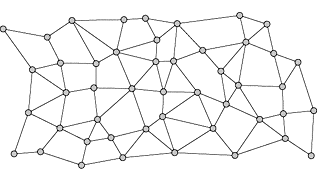
\includegraphics[scale=0.45]{distrib}
\captionsetup{labelformat=empty}
 \caption{La red P2P es una red distribuida, ni centralizada ni descentralizada.}
\end{figure}

Los Bitcoins se crean a partir de un tipo de transacción especial, la transacción de generación, que se incluye en cada bloque. Dicha transacción tiene una dirección de destino (que pertenece al minero que se ha generado el bloque) pero no tiene ninguna dirección de origen. 

Actualmente, pues como veremos esta cantidad va decreciendo, se premia $12.5$ BTC al minero o pool (agrupación de mineros que trabaja en conjunto) que resuelve el bloque. Más adelante explicaremos en profundidad en qué consiste la minería.

Como hemos visto antes, el funcionamiento básico de Bitcoin se basa en las transacciones. Estas se envían de una dirección a otra a través de los nodos, que son los encargados de validar -mediante los mineros- las transacciones y almacenarlas en la blockchain. Ahora explicaremos todas estas funciones de forma detenida.

Además de validar las transacciones, es necesario crear los bloques que las afianzan. Este proceso es el que permite construir el registro común único  -la cadena de bloques- y se realiza de manera totalmente distribuida en Bitcoin. El afianzamiento en Bitcoin se basa en una \textbf{prueba de trabajo} (proof-of-work). 
\begin{defi} Un \textbf{sistema de prueba de trabajo} o \textbf{POW} es un sistema que requiere que el cliente del servicio realice algún tipo de trabajo que tenga cierto coste y que es verificado fácilmente en la parte del servidor. Normalmente el trabajo consiste en realizar un cómputo en el ordenador del cliente. En el caso de Bitoin, el sistema de prueba de trabajo permite la transferencia de valor de manera directa entre los participantes de una transacción sin necesidad de depender de ninguna organización central de confianza. 
\end{defi}
Esta validación puede ocurrir simultáneamente con varios bloques, en cuyo caso se formaría una rama y se continúa a partir del bloque que llega primero.
\begin{figure}[h!]
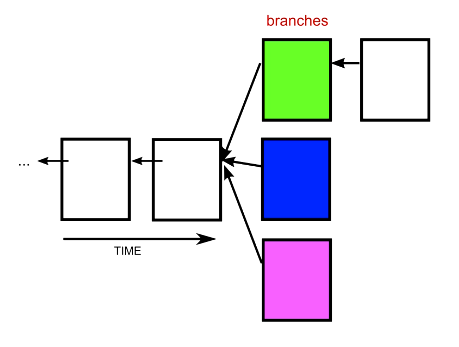
\includegraphics[scale=0.45]{rama}
\end{figure}

¿En qué consiste dicha prueba? La prueba de trabajo que utiliza Bitcoin consiste en encontrar un valor de nonce para el nuevo bloque de tal manera que el
hash del bloque sea inferior a un valor objetivo fijado. Si H es la función hash, lo que un minero es buscar un valor de un nonce tal que:
\[
H(H(Data+Nonce)) < Dif
\]
La dificultad es un valor que se ajusta en función de la capacidad computacional de la red. Por las propiedades de las funciones hash, la unica manera de conseguir un hash inferior al valor objetivo es ir probando diferentes valores de nonce, hasta dar con uno que genere el hash buscado. De este modo, si un atacante quiere modificar la cadena de bloques, ya sea para anular transacciones, ya sea para tener control de lo que se anota en el registro común, necesitará un poder computacional superior al $50\%$ de la red. La red computacional de Bitcoin es la más potente que existe en el mundo, por encima de Google o la NSA.

¿Y cómo varía la dificultad del problema? Como se busca un nonce tal que $H(H(Data+Nonce)) < Dif$, bastará con fijar un valor de $Dif$ cada vez más pequeño. En la representación hexadecimal del hash (o en otra cualquiera) esto se consigue eligiendo una cadena de caracteres que empiece por una determinada cantidad de ceros. Cuantos más ceros, más pequeño es el valor, por lo que a grandes rasgos se trata de buscar el valor del nonce que te dé un hash con la cantidad buscada de ceros iniciales. 

\begin{ej} Vamos a ver un ejemplo simplificado de cómo se construye un bloque. Para ello vamos a usar hashes reducidos, en lugar de los reales de 40 caracteres. Supongamos que el valor del hash del anterior bloque es $00000000000001adf44c7d69767585$ (comienza con 13 ceros). Consideremos dos hashes de transacciones esperando a ser incluidas en el bloque $5572eca4dd4$ y  $db7d0c0b845$. Por último sea el hash de la transacción por la cual el minero intenta recibir recompensa $916d849af76$. El nuevo bloqué tendrá todos los hashes mencionados de la siguiente forma: 
$$00000000000001adf44c7d69767585--5572eca4dd4-db7d0c0b845-916d849af76--$$
Solo falta completarlo con el valor adecuado de nonce. Por ejemplo empezamos con el valor $nonce=1$, con el que resultaría el bloque
$$00000000000001adf44c7d69767585--5572eca4dd4-db7d0c0b845-916d849af76--1$$
Al aplicarle el hash nos da como resultado 
$$8b9b994dcf57f8f90194d82e234b72ac$$
que no puede ser válido porque tiene menos de de 13 ceros (ninguno de hecho). Podemos continuar probando hasta llegar al nonce adecuado. Si somos los primeros en encontrarlo, se añadirá nuestro bloque y recibiremos la recompensa.

\end{ej}


\begin{figure}[h!]
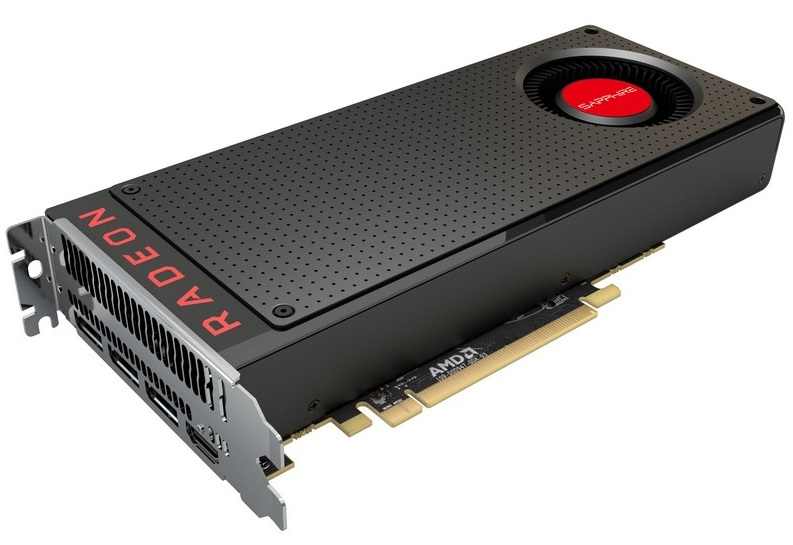
\includegraphics[scale=0.15]{grafica}
\captionsetup{labelformat=empty}
 \caption{La gráfica RX 480 8GB GDDR5 permite minar a  29 MH/s.}
\end{figure}


\begin{figure}[h]
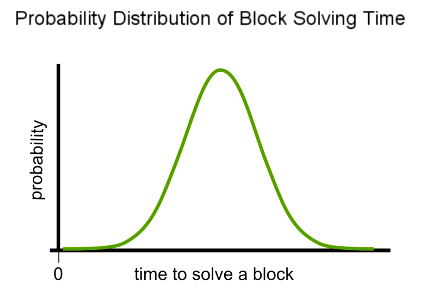
\includegraphics[scale=0.45]{distribution}
\captionsetup{labelformat=empty}
 \caption{La resolución de un bloque ocurre, más o menos, cada diez minutos.}
\end{figure}

\newpage
\subsection{Almacenamiento}
Como hemos visto cuando hemos hablado acera de la blockchain, el almacenaje de la cadena de bloques se lleva a cabo con mucha redundancia pues todos los nodos completos de la red contienen una copia entera de la cadena de bloques (y sus transacciones). Esto permite a estos nodos validar de manera
correcta cada nueva transacción. Tener que mantener una copia completa de la cadena puede suponer un problema para los nodos operando en dispositivos
ligeros como, por ejemplo, dispositivos móviles. En Febrero de 2014, después de 5 años de operaciones con Bitcoin, la cadena de bloques ocupaba unos 13 GB. El día 17 de Mayo de 2017 ocupaba 115 GB.
\begin{figure}[h]
\includegraphics[scale=0.45]{captura}
\captionsetup{labelformat=empty}
 \caption{Evolución del peso en MB de la blockchain de BTC.}
\end{figure}
Aunque de momento no se ha implementado ninguna solución, se discute activamente la posibilidad de incorporar un algoritmo de poda de la cadena, de manera que no sea necesario guardar todas las transacciones. Así, transacciones antiguas podrían ser eliminadas, guardando de ellas solo su hash, para preservar la integridad de la cadena.
\newpage
\subsection{Halving}
El sistema de Bitcoin ha sido diseñado de modo que la recompensa por minar se reduce a la mitad cada 210000 bloques. Este proceso se conoce como \textbf{Halving} o \textbf{Halvening}. Cuando el bloque 0 (conocido como \emph{bloque génesis}) fue minado a principios de 2009 la recompensa fue de 50 BTC. El primer Halving tuvo lugar a finales de 2012, con lo que la recompensa fue de 25 BTC. El último Halvening se produjo en 2016, por lo que actualmente la recompensa es de 12,5 BTC. 

En la introducción comentamos que la cantidad de Bitcoin que se podrá minar es fija (concretamente 21 millones de BTC), y aunque el motivo de trasfondo es puramente económico, está directamente relacionado con el Halving. La explicación se encuentra en la progresión geométrica que sigue la recompensa. 

\begin{defi}
Una progresión geométrica es una sucesión construida de forma recursiva como:
\begin{align*}
&x_0=a\in\R\\
&x_n=rx_{n+1}, r\in\R .
\end{align*}
\end{defi}

En el caso de las recompensas por minar Bitcoin, $r=\frac{1}{2}$ y $a=50\cdot 210000$ (el total de Bitcoins emitidos mientras la recompensa era de 50 BTC). \begin{prop}
La suma de una progresión geométrica en la que $0<r<1$ tiene la siguiente fórmula que no vamos a probar:
\[
S=\sum_{n=0}^{+\infty}x_n=\frac{a}{1-r}.
\]
\end{prop}

Aplicando esto a Bitcoin obtenemos precisamente $S=\frac{10500000}{\frac{1}{2}} = 21000000$. Nótese que la cantidad total de Bitcoin no llegará a ser exactamente 21 millones (concretamente será 20999999.97480000 BTC, esto es, 2520000 Satoshis menos de los 21 millones de BTC) pues la cantidad mínima con la que se puede recompensar es con $10^{-8}$ BTC = 1 Satoshi. De hecho se puede calcular cuándo se empezará a recompensar con 1 Satoshi, lo cual será al acanzar el bloque 6720000. Por lo tanto, a partir del bloque 6930000 no habrá recompensa en absoluto. Cuando ese momento llegue, no se crearán más Bitcoins y los mineros solo obtendrán beneficios a través de comisiones en las transacciones. Para entonces se espera que el valor del Bitcoin sea tan alto que estas comisiones sean más que suficientes para compensar a los mineros.\\

No solo se conoce la cantidad máxima que habrá de Bitcoin, sino también cuándo se alcanzará esta cantidad. Como hemos visto en la sección de minería, el sistema ha sido diseñado para que se produzca aproximadamente un bloque cada 10 minutos. Para ello, a medida que la capacidad computacional de la red aumenta, también se incrementa la dificultad de generar los bloques. ¿Por qué 10 minutos? En realidad esta cantidad es arbitraria y cada criptodivisa establece el suyo, pero tiempos demasiado cortos podrían generar inestabilidad y tiempos muy largos retrasarían las confirmaciones. 

Un bloque cada 10 minutos supone unos 144 bloques por día. Así que el tiempo para alcanzar 6930000 se necesitan $\frac{6930000}{144} = 48125$ días, algo menos de 132 años. Esto quiere decir que en torno al año 2140 se habrán minado todos los Bitcoins previstos.





\vspace{5cm}

\newpage
\section{Problema de los generales bizantinos}
El problema de los generales bizantinos es un experimento mental creado para ilustrar el dilema de lograr un consenso entre un conjunto de entidades con un objetivo común cuando entre ellas pueden existir traidores, es decir, entidades con objetivos opuestos que intenten dinamitar el proceso. Ademas, se supone que las comunicaciones entre dichas entidades son limitadas e inseguras. 
\begin{problem}
El problema se presenta como una analogía con un escenario de guerra, donde un grupo de generales bizantinos se encuentran acampados con sus tropas alrededor de una ciudad enemiga que desean atacar. Después de observar el comportamiento del enemigo, los generales deben comunicar sus observaciones y ponerse de acuerdo en un plan de batalla común que permita atacar la ciudad y vencer. Para ello, los generales se comunican únicamente a través de mensajeros. 

Existe la posibilidad que algunos de los generales sean traidores y, por lo tanto, decidan enviar mensajes con información errónea con el objetivo de confundir a los generales leales. Un algoritmo que solucione el problema debe asegurar que todos los generales leales acuerdan un mismo plan de accion y que unos pocos traidores no pueden conseguir que el plan adoptado por los generales leales sea equivocado.
\end{problem}
El desarrollo que hemos efectuado acerca de la blockchain su tecnología impide que una persona o un grupo pueda crear bloques falsos es considerada como la primera solución práctica al problema. 

\newpage 
\section{Aplicaciones de la Blockchain}
Terminamos este trabajo mencionando algunas aplicaciones de la tecnología fundamental bajo Bitcoin: la Blockchain. 
\begin{itemize}
\item \textbf{Gestión de identidades}. La tecnología blockchain permite a los usuarios crear su propia identidad digital a prueba de manipulación. Según los expertos, esta especie de ID basado en blockchain reemplazará pronto a los nombres de usuario y contraseñas en línea.

Podremos utilizar nuestra identidad blockchain para acceder a aplicaciones y sitios web, firmar documentos digitales, etc. Ya hay algunas compañías que ofrecen este tipo de servicios, como: Onename, Keybase o ShoCard.

\item \textbf{Alquiler de propiedades y economía colaborativa}. El sistema anterior se puede hacer aún más complejo combinándolo con un contrato inteligente de alquiler. Por ejemplo, si un propietario de un piso o un vehículo quiere alquilarlo, bastaría con elaborar y almacenar en la blockchain un contrato inteligente en el que el propietario fija un precio para el alquiler por un tiempo.

En el momento en que el usuario realiza el pago con una transacción registrada en la blockchain, el contrato inteligente se ejecutaría permitiendo el acceso a la propiedad a dicho usuario concreto por el tiempo estipulado. Una compañía que ofrece este tipo de servicios es Slock.

\item\textbf{Votar por Internet}. La blockchain resuelve uno de los grandes problemas de los sistemas de votación por Internet: el anonimato del voto.

Por su propia estructura y funcionamiento, la blockchain puede garantizar que una persona no pueda votar más de una vez en una misma elección, al tiempo que garantiza la privacidad de su voto. Además, al no haber ninguna autoridad central que gestione la votación no es posible manipularla.

El voto electrónico mejoraría la rapidez y abarataría considerablemente el coste de unas elecciones y referéndums, lo que permitiría hacer referéndums con más frecuencia y mejorar así la democracia.

\end{itemize}
\newpage
\addcontentsline{toc}{section}{Bibliografía}

\begin{thebibliography}{}
\bibitem{Bizant} Cristina Pérez-Solà \& Jordi Herrera-Joancomartí, \textit{Bitcoins y el problema de los generales bizantinos}, 2014. \url{https://web.ua.es/en/recsi2014/documentos/papers/bitcoins-y-el-problema-de-los-generales-bizantinos.pdf}
\bibitem{Khan} Kahn Academy. \url{https://www.khanacademy.org/economics-finance-domain/core-finance/money-and-banking/bitcoin/v/bitcoin-what-is-it}
\bibitem{wiki} Bitcoinwiki, \url{https://en.bitcoin.it/wiki/How_bitcoin_works}.
\bibitem{Eric} Eric Rywalder, \textit{The math behind Bitcoin}, Coindesk, 2014.\\ \url{http://www.coindesk.com/math-behind-bitcoin/}
\bibitem{Alex} Alex Gorale, \textit{Explaining the math behind Bitcoin.} Cryptocoinsnews, 2014.\\ \url{https://www.cryptocoinsnews.com/explaining-the-math-behind-bitcoin/}
\bibitem{youtube} Scott Driscoll, \textit{How Bitcoin works under the hood}. ImponderableThings, 2013. \url{http://www.imponderablethings.com/2013/07/how-bitcoin-works-under-hood.html}
\bibitem{Halving} Bitcoin Forum, \url{https://bitcointalk.org/index.php?topic=1473285.0}
\end{thebibliography}



\end{document}